\chapter{Crowdsourcing strategies in Pl@ntNet citizen based learning platform}
\label{chap:plantnet}
\enlargethispage{3\baselineskip}

\begin{keypointstwomargins}{Pl@ntNet}{-2cm}{-1cm}
        \textbf{Key points -- Crowdsourcing plant species}
        \begin{enumerate}[leftmargin=*]
        \item Aiding botanists in plant species identification is a challenging task. Species are often visually close and their identification requires expert knowledge.
        \item Pl@ntNet is a citizen science platform that allows users to upload images of plants and receive a list of possible species.
        \item The collaborative aspect of Pl@ntNet allows users to vote on the species they think are present in the image and contribute to new labeled data, which is then used to train a computer vision and help new identifications.
        \end{enumerate}

        \textbf{Contributions -- Exploration of Pl@ntNet label aggregation strategy}
        \begin{enumerate}[leftmargin=*,start=4]
        \item We release and evaluate the current Pl@ntNet label aggregation and compare it to other strategies.
        \item We release a subset of Pl@ntNet with images url and collected labels in the South Western European Flora of more than $6$ million observations and $800$ thousand users in a large-scale classification setting.
        \item We discuss how to integrate the current model's predictions in the votes aggregation. This is a challenging task due to the iterative aspect of Pl@ntNet: the current data helps train the next generation of models iteratively.
        \end{enumerate}
\end{keypointstwomargins}


\section{Crowdsourcing for plant species identification}

Computer vision models are a great aid in plant species recognition in the field \citep{vidal2021perspectives,borowiec2022}.
However, to train them we need large annotated datasets.
These datasets are often created thanks to citizen science approaches, collecting both reliable and useful information \citep{brown2019potential}.
Among existing plant recognition applications, the Pl@ntNet citizen science platform \citep{affouard2017pl} enables global data collection by allowing users to upload and annotate plant observations.

\begin{figure}[htb]
    \centering
    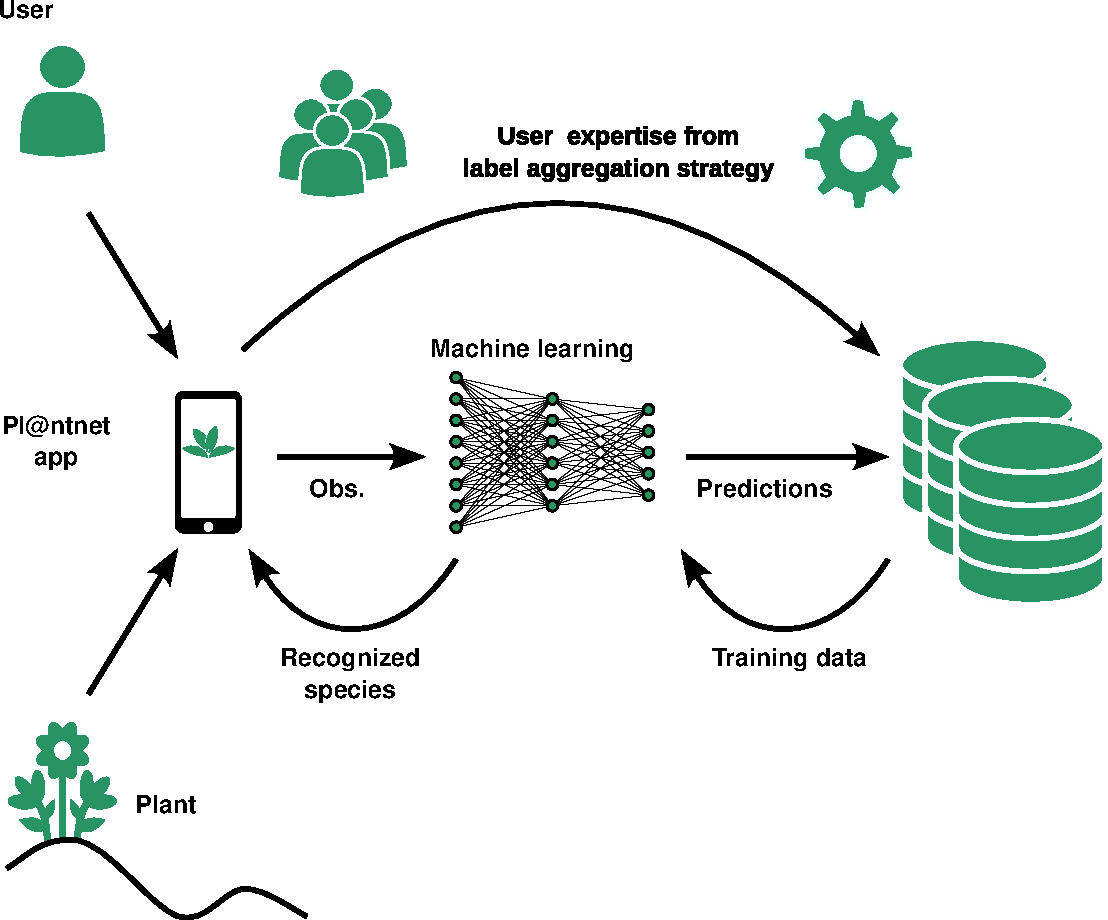
\includegraphics[width=.75\linewidth]{images/plantnet_schema_global_green.pdf}
    \caption{Pl@ntNet system of human-AI interaction for plant species recognition. Users take their plant observations in the Pl@ntNet application. A prediction is output by the AI model. Users can validate the prediction or propose another species. The whole votes collection is used to evaluate user expertise and actively revise observations identifications.}
    \label{fig:plantnet-system}
\end{figure}

\subsection{Plant taxonomy generalities}
First, we need to understand the complexity of plant taxonomy.
Our goal here is to briefly present the taxonomy of plants.
Plants are divided following a hierarchy, from the most general to the most specific ranks of taxa: kingdom, division, class, order, family, genus, and species according to the International Code of Nomenclature for algae, fungi and plants (ICN) \citep{turland2018international}.
Each of these units of biological classification is called a taxon (taxa in plural).
Further secondary ranks also exist (tribe, subspecies, variety, form) but we will focus on the main ones.

Roughly, an example of taxonomy levels is:
\begin{itemize}
        \item Kingdom: separates plants from animals, fungi, and bacteria -- \emph{e.g} Plantae.
        \item Division: separates spore (\emph{angiosperms}) or seed (\emph{gymnosperms}) reproduction with specific characteristics. There are 14 plant divisions in total.
        \item Class: Angiosperms are divided into Monocotyledons(grasses, yuccas, etc.) and Dicotyledons (angiosperms with pair of leaves).
        \item Order: Group of families with common characteristics -- \emph{e.g} \emph{Cucurbitales} (generally ends with \emph{-ales}).
        \item Family: Plants with similar flower, fruit and seed structures -- \emph{e.g} \emph{Begonaias and Allies}.
        \item Genus: First part of the plant's scientific name (capitalized and italicized) -- \emph{e.g} \emph{Begonia}.
        \item Species: a group of organisms capable of producing fertile offspring -- \emph{e.g} \emph{Begonia ferox}. If the species is unknown it is called \emph{sp.} or \emph{spp.} for plural.
\end{itemize}

XXX TODO: add a figure of the taxonomy of a plant.
XXX TODO: add a figure of my begonia ferox.


A plant name is generally composed of two parts: the genus and the species.


\subsubsection{Checklists and referentials}




\subsubsection{What is a plant observation?}

Contrary to classical datasets, Pl@ntNet observations are not a single image but a set of images taken by a user in the field.
A single image of a plant might not be enough to identify

\subsection{Presenting the voting interface}

\subsection{A step in a bigger pipeline}

\section{Pl@ntNet's label aggregation strategy}

\subsection{Presentation of the algorithm}

\subsection{Presenting a subset of Pl@ntNet to evaluate the current strategy}

\section{Integrating model predictions in the aggregation}

\subsection{Possible strategies}

\subsection{Can we trust our current predicted probabilities?}

\section{Conclusion}